\chapter{LV 7 am 20.06.2014}
\section{Teststrategien}
\paragraph{Beispiel:}
Das hier angeführte Beispiel zeigt die Anwendung der $Nx1$ Strategie für unser Anwendungsbeispiel.\\\\
$<Stm> := <Assign> | <Loop> | <Case>$\\\\
$x12 = (-b +- sqrt(b^2 - 4ac))/2a$\\\\
Des weiteren wies Bernd Wenzel darauf hin, das sich jeder bis zur nächsten Stunde überlegen sollte welche Test mit der $Nx1$ Strategie für unser Beispiel getestet werden müssten. 

\subsection{Überdeckungen}
Ein anderer Ansatz ist die schwache $Nx1$ Strategie. Mit der schwache $Nx1$-Strategie können Grenzverschiebungen erkannt werden. Es werden für jede Unterdomäne und für jede Grenze $n$ linear unabhängige Testpunkte auf der Grenze, ein Testpunkt nicht auf der Grenze, ein Testpunkt außerhalb der Unterdomäne, falls die Grenze abgeschlossen ist, ein Testpunkt innerhalb der Unterdomäne, falls die Grenzen offen sind definiert. Zusätzlich wird ein Testpunkt im Inneren der Unterdomäne definiert. Insgesamt hat man dann $(n+1)*b+1$ Testpunkte pro Unterdomäne mit $b$ Grenzen. Der Aufwand dieser Strategie ist sehr groß, doch sie erkennt dafür Abschlussprobleme, Grenzverschiebungen, fehlende Grenzen und die meisten überflüssigen Grenzen (allerdings nicht alle). 
Eine andere Strategie ist die schwache $1x1$ Strategie. Sie reduziert den hohen Aufwand der $Nx1$ Strategie ohne dabei gravierende Qualitätseinbußen zu haben. Sie erkennt Abschlussprobleme, die Grenzverschiebungen werden meistens vermieden. Es werden fehlende Grenzen erkannt. Sie bietet einen guten wirtschaftlichen Kompromiss.


\subsection{Endliche Automaten und Markov-Modelle}
Die meisten Anwendungsprogramme lassen sich als endliche Automaten mit Ausgabe darstellen. Man versucht auf eine beherrschbare Anzahl an Zustände und Übergänge zu erreichen. Für die Vereinfachung ist es notwendig, die Anzahl der Zustände deutlich kleiner als 100 zu halten. Viele sagen, dass 7 Zustände schon zu viel seien. Für Webapplikationen bietet sich diese Methode zum Testen sehr gut an, da jede Seite als eigener Zustand definiert werden kann. Man kann eine Beschränkung für nur relevante Seiten definieren, wodurch sich die Anzahl der Zustände verringert. 

Man muss die Zustände, Übergänge und die I/O-Beziehungen definieren um das Model zu validieren. Für die Testziele ist es relevant zu bewerten, ob alle Zustände erreichbar, vollständig und notwendig sind. Bei den Übergängen ist die Durchführbarkeit  ein wichtiger Punkt. Hier sollte darauf geachtet werden, dass keine Wiederholung der Prüfung der Zustandserreichbarkeit der bereits ausgeführter Übergänge stattfindet. 

Diese Endlichen Automaten können mittels eines Markov-Modelsl (auch Markov-Kette) getestet werden. Es wird ein endlicher Automat mit Wahrscheinlichkeiten an jedem Zustandsübergang erstellt. Bei einem unvollständigen Modell ist die Summe der Wahrscheinlichkeiten aller ausgehenden Übergänge < 1. Dann handelt es sich dabei um ein unvollständiges Modell. Eine weitere Ausprägung davon stellt das UMM (Unified Markov Model) da.

Die Wahrscheinlichkeit eines konkreten Übergangs ist das Produkt aller Wahrscheinlichkeiten auf dem Pfad vom Start bis zum Ausgangszustand, multipliziert mit der Wahrscheinlichkeit dieses konkreten Übergangs. Bei Schleifen kann dies unangenehm werden.

Das Unified Markov Model (UMM) ist ein kohärenter Satz von hierarchisch geschachtelten Markov-Modellen und ist deutlich besser in der Praxis einsetzbar als das Markov-Modell. Es eignet sich vor allem für alle Arten von statistischen Aussagen (z.B. Zuverlässigkeit, Verfügbarkeit, ...).

\subsection{Kontrollfluss}
Beim Kontrollfluss ist das Testziel die Ausführung aller Pfade im Programm. Der Control Flow Graph (CFG) besteht aus Knoten, welche ausführbare Anweisungen sind (Unterscheidung zwischen Startknoten und Endknoten), und Kanten, welche mögliche Verarbeitungssequenzen darstellen. 

Prinzipiell wird versucht alle Pfade auszuführen. Lediglich Schleifen sind davon ausgenommen, da sie ein Problem darstellen. Es musst bei Schleifen getestet werden:
\begin{itemize}
\item komm ich überhaupt in die Schleife rein
\item funktioniert sie mit einer, zwei, drei,... Durchläufen
\item erreiche ich die Grenzfälle
\end{itemize}

Die Empfehlung hier ist es, den Pfad von hinten aufzubauen, da so die Identifikation von nicht benötigtem Code unterstützt wird.

\subsection{Datenfluss}
Beim Data Dependency Graph (DDG) stellen Knoten Zustände von Variablen dar und die Kanten stehen für die Operationen des Programms. 
\begin{figure}[hbtp]
\centering
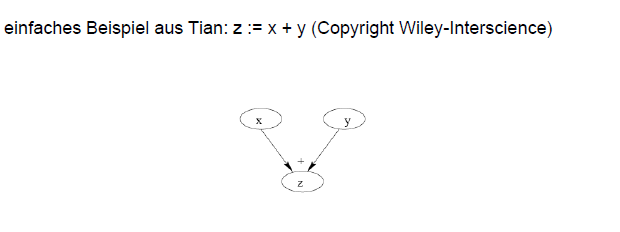
\includegraphics[scale=0.8]{document/graphics/DDG} 
\caption{DDG}
\end{figure}

Beim DDG wird die Art des Zugriffs auf einen Zustand unterschieden. Es gibt einen lesenden und einen schreibenden Zugriff. Somit ist es möglich Zugriffsfolgen zu definieren, die Probleme darstellen könnten. Zum Beispiel geht von einem Schreib-Lese-Zugriff (S-L) oder einem Lese-Lese-Zugriff keine potentielle Gefahr aus. Ein Schreib-Schreib-Zugriff deutet allerdings auf mögliche Fehler und Ineffizienz hin. 

\section{Testverfahren}
Bei den Testverfahren haben wir gelernt aus was ein Testverfahren besteht und in welchen Phasen der Entwicklung welche Testtypen zur Anwendung kommen.
Einer dieser Testtypen ist der Unit-Test.
Bei den Unit Tests wird ein White Box Test durch den Entwickler realisiert. Es handelt sich dabei um informelles Testen um Fehler zu lokalisieren. 
Eine andere Art ist der Komponenten-Test.
Bei einem Komponenten-Test wird entweder ein White Box Test oder Black Box Test durch den Entwickler realisiert. White Box Tests werden hier eher für prozedurale Sprache verwendet und Black Box Tests vor allem OO-Sprachen.
Bei einem Integrationstest wird ein Black Box Test in Bezug auf die zu integrierenden Komponenten und ein White Box Test in Bezug auf die Integrationsschicht (durch Entwickler) durchgeführt. 

Bei einem Systemtest werden Black Box Tests durch professionelle Tester durchgeführt.

Des weiteren gibt es noch Regressionstests, Abnahmetests und Betatests. 

Dort wo Black Box Tests durchgeführt werden, spielen Checklisten, Benutzungsprofile, Endliche Automaten eine wichtige Rolle. Bei den White Box Tests ist überdeckungsbasiertes Testen und ein Kontrollfluss wichtig. 

\section{Testwerkzeuge}
\subsection{Debugger}
Debuggen bedeutet nicht Testen! Debuggen kann allerdings zum Testen verwendet werden um beispielsweise den für einen Test benötigten Status herzustellen. Ein großer Vorteil ist, dass wir uns so nicht zum planlosen Probieren verführen lassen.

\subsection{Ausführbare Tests}
Dabei handelt es sich um automatisierte Tests. Um das zu realisieren gibt es zum Beispiel JUnit (Java, C), NUnit (CSharp), CPPUnit (C++), JSUnit (JavaScript), PHPUnit (PHP) etc.
Hierbei ist wichtig das sich der Testcode und das SuT gegenseitig testen.
 
\subsection{Testrahmen}
Wichtig ist es denn richtigen Testrahmen zu erstellen. Hierbei sind vor allem Komponenten wie SuT, Testframe und Testplan wichtig. Die Tests können im Bottom-Up Prinzip abgearbeitet werden.

\subsection{Emulatoren/Simulatoren}
\paragraph{Simulator}
Vereinfachtes Modell eines Systems zum Zweck der Analyse dieses Systems.
\paragraph{Emulator}
Nachbildung wesentlicher Verhaltensaspekte eines Systems durch ein anderes.

Simulatoren und Emulatoren finden in verschiedenen Bereichen Anwendung. Ein Beispiel wäre dabei EADS-Astrium

\subsection{Überdeckungsanalyse}
Nach der Durchführung eines White-Box Tests muss eine Messung der Testüberdeckung auf Ebene der Anweisungen erfolgen. Dies erfordert allerdings eine Instrumentierung des Codes. Beispiel eines solchen Systems wäre Cobertura.

\subsection{GUI Capture/Replay}
Hierbei handelt es sich um ein Testverfahren über eine Grafische Oberfläche. Hierbei müssen Werkzeuge verwendet werden, die diese Tests automatisiert. Diese Werkzeuge werden Capture und Replay Werkzeuge genannt. Laut Bernd Wenzels Beobachtungen macht das Testen über ein solches System keinen Spaß. 

TODO bis Seite 105 DANKE THOMAS